\documentclass[t]{beamer}
\mode<presentation>

\usepackage{etex}

\usetheme{Madrid}
% other themes: Warsaw, AnnArbor, Antibes, Bergen, Berkeley, Berlin, Boadilla, boxes, CambridgeUS, Copenhagen, Darmstadt, default, Dresden, Frankfurt, Goettingen,
% Hannover, Ilmenau, JuanLesPins, Luebeck, Madrid, Maloe, Marburg, Montpellier, PaloAlto, Pittsburg, Rochester, Singapore, Szeged, classic

\setbeamertemplate{navigation symbols}{\insertslidenavigationsymbol}

\usecolortheme{dolphin}
%\usecolortheme{seagull}
% color themes: albatross, beaver, beetle, crane, default, dolphin, dov, fly, lily, orchid, rose, seagull, seahorse, sidebartab, structure, whale, wolverine

%\usefonttheme{serif}
% font themes: default, professionalfonts, serif, structurebold, structureitalicserif, structuresmallcapsserif

% pdf is displayed in full screen mode automatically
%\hypersetup{pdfpagemode=FullScreen}

%\AtBeginSection[]
%{
%  \begin{frame}<beamer>
%    \frametitle{Outline}
%    \tableofcontents[currentsection,currentsubsection]
%  \end{frame}
%}

% define your own colours:
\definecolor{Red}{rgb}{1,0,0}
\definecolor{Blue}{rgb}{0,0,1}
\definecolor{Green}{rgb}{0,1,0}
\definecolor{magenta}{rgb}{1,0,.6}
\definecolor{lightblue}{rgb}{0,.8,1}
\definecolor{lightpurple}{rgb}{.6,.4,1}
\definecolor{gold}{rgb}{.6,.5,0}
\definecolor{orange}{rgb}{1,0.4,0}
\definecolor{hotpink}{rgb}{1,0,0.5}
\definecolor{newcolor2}{rgb}{.5,.3,.5}
\definecolor{newcolor}{rgb}{0,.3,1}
\definecolor{newcolor3}{rgb}{1,0,.35}
\definecolor{darkgreen1}{rgb}{0, .35, 0}
\definecolor{darkgreen}{rgb}{0, .6, 0}
\definecolor{darkred}{rgb}{.75,0,0}

\xdefinecolor{olive}{cmyk}{0.64,0,0.95,0.4}
\xdefinecolor{purpleish}{cmyk}{0.75,0.75,0,0}

%\usepackage{beamerinnerthemerounded}
% inner themes include circles, default, inmargin, rectangles, rounded

%\usepackage{beamerouterthemesmoothbars}
% outer themes include default, infolines, miniframes, shadow, sidebar, smoothbars, smoothtree, split, tree

\useoutertheme[subsection=false]{smoothbars}

% to have the same footer on all slides
\setbeamertemplate{footline}[text line]{
  %
\includegraphics[height=15pt]{sulogo.eps}
  \hfill 
\raisebox{5pt}{Math 207:  Introduction to Statistics}\hfill 
\raisebox{5pt}{The Normal Curve and  Normal Approximation for Data}\hfill
\raisebox{5pt}{\insertframenumber/\pageref{lastpage}}}
%\setbeamertemplate{footline}[text line]{} % or empty footer

% include packages
\usepackage{subfigure}
\usepackage{multicol}
\usepackage{amsmath}
\usepackage{epsfig}
\usepackage{graphicx}
\usepackage[all,knot]{xy}
\xyoption{arc}
\usepackage{url}
\usepackage{multimedia}
\usepackage{hyperref}
\usepackage{setspace}

\title{Math 207:  Introduction to Statistics}
\subtitle{The Normal Curve and Normal Approximation for Data}
\author{Ralph Wojtowicz}
\institute{Department of Mathematics\\ Shenandoah}
%\date{\scriptsize 25 January 2012}

\usepackage{pstricks,pst-grad,pst-func,pst-text,pst-node,multido,pst-plot,calc,pst-3dplot}

\newcommand{\BRACE}{
\begin{pspicture}(-3,-2.1)(3,1.1)
\psset{yunit=3,linewidth=0.02}
\psline(-3.5,0)(3.5,0)  
  \psline(-3,0)(-3,-0.04) \rput[t](-3,-0.07){\scriptsize -3\hphantom{-}}
  \psline(-2,0)(-2,-0.04) \rput[t](-2,-0.07){\scriptsize -2\hphantom{-}}
  \psline(-1,0)(-1,-0.04) \rput[t](-1,-0.07){\scriptsize -1\hphantom{-}}
  \psline(0,0)(0,-0.04)   \rput[t](0,-0.07){\scriptsize 0}
  \psline(1,0)(1,-0.04)   \rput[t](1,-0.07){\scriptsize 1}
  \psline(2,0)(2,-0.04)   \rput[t](2,-0.07){\scriptsize 2}
  \psline(3,0)(3,-0.04)   \rput[t](3,-0.07){\scriptsize 3}
  \rput[l](3.6,0){\scriptsize $x$}
\psline(0,0)(0,0.5)
  \psline(-0.12,0.5)(0,0.5)    \rput[r](-0.21,0.5){\scriptsize $0.5$}
  \psline(-0.12,0.25)(0,0.25)  \rput[r](-0.21,0.25){\scriptsize $0.25$}
\psGauss[linecolor=blue,linewidth=0.02,sigma=1,mue=0]{-3}{3}
\pnode(-1,-0.15){A}\pnode(1,-0.15){B}
\psbrace[braceWidth=0.02,braceWidthInner=5pt,braceWidthOuter=5pt](A)(B){\rput{90}(0.25,-0.05){\scriptsize 68\%}}
%
\pnode(-2,-0.15){C}\pnode(2,-0.15){D}
\psbrace[braceWidth=0.02,braceWidthInner=25pt,braceWidthOuter=5pt](C)(D){\rput{90}(0.25,-0.05){\scriptsize 95\%}}
%
\pnode(-3,-0.15){E}\pnode(3,-0.15){F}
\psbrace[braceWidth=0.02,braceWidthInner=45pt,braceWidthOuter=5pt](E)(F){\rput{90}(0.25,-0.1){\scriptsize 99.7\%}}
\end{pspicture}}

\begin{document}

%\frame[plain]{
%	\titlepage
%}


\begin{frame}[plain]
\definecolor{myblue}{rgb}{0,0,0.6}
\definecolor{grayA}{rgb}{0.95,0.95,0.95}
\definecolor{grayB}{rgb}{0.98,0.98,0.98}
\begin{center}

%\begin{pspicture}(0,0)(7,4.8)
\begin{pspicture}(-6,-7)(6,2)
\rput(0,-1.85){\scalebox{0.95}{\BRACE}}%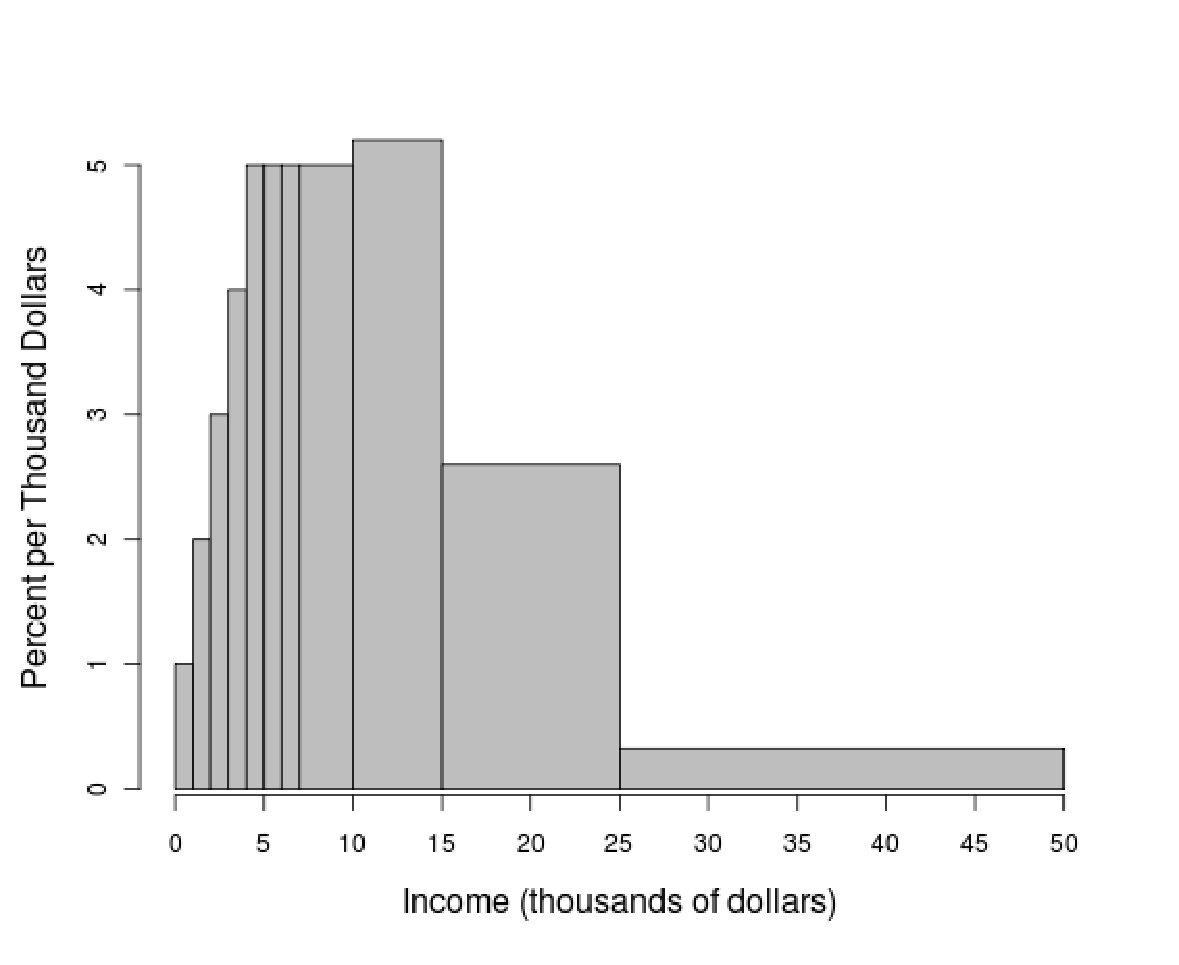
\includegraphics[height=1.8in]{../Fig4p37.eps}}
\psframe[linewidth=0.02,linecolor=gray](-6.2,-7)(6.2,2.2)
\psframe[linewidth=0.02,linecolor=gray](-6.15,-6.95)(6.15,2.15)
\rput(0,1.4){\color{myblue}\large Math 207:  Introduction to Statistics}
\rput(0,0.6){\color{myblue}The Normal Curve and Normal Approximation to Data}
%\psframebox(0,0)(4,4)
\rput(0,-4.4){\scriptsize Dr.~Ralph Wojtowicz}
\rput(0,-4.9){\scriptsize Mathematics Department}
\rput(0,-5.8){
\includegraphics[height=1cm]{sulogo.eps}}
%
%\rput(0,-6.5){\scriptsize 25 January 2012}
\end{pspicture}
\end{center}

\end{frame}

%\section[Outline]{}

\addtocounter{page}{-1}
\addtocounter{framenumber}{-1}

{\footnotesize
\frame{\tableofcontents}
}

\section{The Normal Curve}
\subsection{The Normal Curve}
\begin{frame}[t]\frametitle{The Normal Curve}

{\small

\begin{itemize}
\item The {\color{blue}\textbf{standard normal}}
 (or Gaussian) curve is an ideal histogram to which
  we will compare other data.
\end{itemize}
\begin{center}
\begin{pspicture}(-3,-2.1)(3,1.1)
\psset{yunit=3,linewidth=0.02}
\psline(-3.5,0)(3.5,0)  
  \psline(-3,0)(-3,-0.04) \rput[t](-3,-0.07){\scriptsize -3\hphantom{-}}
  \psline(-2,0)(-2,-0.04) \rput[t](-2,-0.07){\scriptsize -2\hphantom{-}}
  \psline(-1,0)(-1,-0.04) \rput[t](-1,-0.07){\scriptsize -1\hphantom{-}}
  \psline(0,0)(0,-0.04)   \rput[t](0,-0.07){\scriptsize 0}
  \psline(1,0)(1,-0.04)   \rput[t](1,-0.07){\scriptsize 1}
  \psline(2,0)(2,-0.04)   \rput[t](2,-0.07){\scriptsize 2}
  \psline(3,0)(3,-0.04)   \rput[t](3,-0.07){\scriptsize 3}
  \rput[l](3.6,0){\scriptsize $x$}
\psline(0,0)(0,0.5)
  \psline(-0.12,0.5)(0,0.5)    \rput[r](-0.21,0.5){\scriptsize $0.5$}
  \psline(-0.12,0.25)(0,0.25)  \rput[r](-0.21,0.25){\scriptsize $0.25$}
\psGauss[linecolor=blue,linewidth=0.02,sigma=1,mue=0]{-3}{3}
\pnode(-1,-0.15){A}\pnode(1,-0.15){B}
\psbrace[braceWidth=0.02,braceWidthInner=5pt,braceWidthOuter=5pt](A)(B){\rput{90}(0.25,-0.05){\scriptsize 68\%}}
%
\pnode(-2,-0.15){C}\pnode(2,-0.15){D}
\psbrace[braceWidth=0.02,braceWidthInner=25pt,braceWidthOuter=5pt](C)(D){\rput{90}(0.25,-0.05){\scriptsize 95\%}}
%
\pnode(-3,-0.15){E}\pnode(3,-0.15){F}
\psbrace[braceWidth=0.02,braceWidthInner=45pt,braceWidthOuter=5pt](E)(F){\rput{90}(0.25,-0.1){\scriptsize 99.7\%}}
\end{pspicture}
\end{center}
\begin{itemize}
\item The total area under the curve is $1$ (or $100$\%).
\item The curve is symmetric about the line $x=0$.
\item It has $\mbox{mean}=0$ and $\mbox{sd}=1$.
\end{itemize}

}

\end{frame}

\subsection{Standard Units}
\begin{frame}[t]\frametitle{Standard Units}
{\small

\begin{itemize}
\item If $x_1$, $\dots$, $x_n$ is a list of numbers, we convert the values
in the list to {\color{blue}\textbf{standard units}} using the following formula:
\vspace{-5pt}
\end{itemize}
\[z_i = \frac{x_i - \mbox{mean}}{\mbox{sd}}\vspace{-12pt}\]
\begin{itemize}
\item $z_i$ measures how far (in units of sd) $x_i$ is from the mean (average) of the list
\item Example:  Consider the list 13, 9, 10, 11, 7, 10.\\
   \texttt{> x <- c(13, 9, 10, 11, 7, 10)}\\
   \texttt{> mean(x)}\\
   \texttt{[1] 10}\\
   \texttt{> sd(x)}\\
   \texttt{[1] 2}\\[5pt]
   Now convert 13 to standard units:\\
   \texttt{> (13-10)/2}\\
   \texttt{[1] 1.5}\\
\end{itemize}
}

\end{frame}

\section[Areas]{Finding Areas Under the Normal Curve}
\subsection{Finding Areas Under the Normal Curve with \texttt{R}}
\begin{frame}[t]\frametitle{Finding Areas Under the Normal Curve with \texttt{R}}

{\small

\begin{center}
\begin{pspicture}(-3,-2.5)(3,1.75)
\psframe[linewidth=0.02](-3.8,-1.1)(4.2,1.8)
\psset{yunit=3,linewidth=0.02}
%
   \pscustom[fillstyle=solid,fillcolor=lightgray,sigma=1,linestyle=none]{
     \psGauss{-3.5}{1.25}
     \psline(1.25, 3.490343)(1.25,0)(-3.5,0) }
   \psGauss[sigma=1,linecolor=blue,linewidth=0.5pt]{-3.5}{3.5}
\psline(1.25,0.1826)(1.25,-0.22)   \rput[t](1.25,-0.25){\scriptsize 1.25}
\rput[l](1.5,0.3){\scriptsize\texttt{pnorm}$(1.25)\approx 0.894$}
\psline{->}(1.45,0.29)(0.5,0.2)
%
\psline(-3.5,0)(3.5,0)  
  \psline(-3,0)(-3,-0.04) \rput[t](-3,-0.07){\scriptsize -3\hphantom{-}}
  \psline(-2,0)(-2,-0.04) \rput[t](-2,-0.07){\scriptsize -2\hphantom{-}}
  \psline(-1,0)(-1,-0.04) \rput[t](-1,-0.07){\scriptsize -1\hphantom{-}}
  \psline(0,0)(0,-0.04)   \rput[t](0,-0.07){\scriptsize 0}
  \psline(1,0)(1,-0.04)   \rput[t](1,-0.07){\scriptsize 1}
  \psline(2,0)(2,-0.04)   \rput[t](2,-0.07){\scriptsize 2}
  \psline(3,0)(3,-0.04)   \rput[t](3,-0.07){\scriptsize 3}
  \rput[l](3.6,0){\scriptsize $x$}
\psline(0,0)(0,0.5)
  \psline(-0.12,0.5)(0,0.5)    \rput[r](-0.21,0.5){\scriptsize $0.5$}
  \psline(-0.12,0.25)(0,0.25)  \rput[r](-0.21,0.25){\scriptsize $0.25$}
\end{pspicture}
%%%
\begin{pspicture}(-3,-2.1)(3,1.1)
\psframe[linewidth=0.02](-3.8,-1.1)(4.2,1.8)
\psset{yunit=3,linewidth=0.02}
%
   \pscustom[fillstyle=solid,fillcolor=lightgray,sigma=1,linestyle=none]{
     \psGauss{-3.5}{0.6744898}
     \psline(0.6744898, 0.3177766)(0.6744898,0)(-3.5,0) }
   \psGauss[sigma=1,linecolor=blue,linewidth=0.5pt]{-3.5}{3.5}
\psline(0.6744898,0.3177766)(0.6744898,-0.22)   
   \rput[tl](0.61,-0.23){\scriptsize\texttt{qnorm}$(0.75)\approx 0.67$}
\rput[l](1.5,0.3){\scriptsize$\mbox{area}=0.75$}
\psline{->}(1.45,0.29)(0.25,0.15)
%
\psline(-3.5,0)(3.5,0)  
  \psline(-3,0)(-3,-0.04) \rput[t](-3,-0.07){\scriptsize -3\hphantom{-}}
  \psline(-2,0)(-2,-0.04) \rput[t](-2,-0.07){\scriptsize -2\hphantom{-}}
  \psline(-1,0)(-1,-0.04) \rput[t](-1,-0.07){\scriptsize -1\hphantom{-}}
  \psline(0,0)(0,-0.04)   \rput[t](0,-0.07){\scriptsize 0}
  \psline(1,0)(1,-0.04)   \rput[t](1,-0.07){\scriptsize 1}
  \psline(2,0)(2,-0.04)   \rput[t](2,-0.07){\scriptsize 2}
  \psline(3,0)(3,-0.04)   \rput[t](3,-0.07){\scriptsize 3}
  \rput[l](3.6,0){\scriptsize $x$}
\psline(0,0)(0,0.5)
  \psline(-0.12,0.5)(0,0.5)    \rput[r](-0.21,0.5){\scriptsize $0.5$}
  \psline(-0.12,0.25)(0,0.25)  \rput[r](-0.21,0.25){\scriptsize $0.25$}
\end{pspicture}

\end{center}
}
\end{frame}

\subsection{Finding Areas Under the Normal Curve}
\begin{frame}[t]\frametitle{Finding Areas Under the Normal Curve}
{\small
\begin{itemize}
\item Use one or more of the following to find areas under the normal curve:
  \begin{itemize}
  \item Total area under the curve is 1 (that is, 100\%)
  \item The area is symmetric about vertical the line $x=0$
  \item (area to the left of $x$) $=$ ($1-\mbox{area to the right of $x$}$)
  \item The 68\%, 95\%, 99.7\% rules (see slide 2)
  \item The \texttt{pnorm} or \texttt{qnorm} functions in \texttt{R}
  \item Normal table in your text
 \end{itemize}
\item Example:  
\end{itemize}}

\begin{center}
\begin{pspicture}(-3,-2.5)(3,1.3)
\psframe[linewidth=0.02](-3.8,-1.1)(4.9,1.8)
\psset{yunit=3,linewidth=0.02}
%
\pscustom[fillstyle=solid,fillcolor=lightgray,sigma=1,linestyle=none]{
     \psGauss{-1}{1.25}
     \psline(1.25, 3.490343)(1.25, 0)(-1, 0)(-1, 0.3678794)}
   \psGauss[sigma=1,linecolor=blue,linewidth=0.5pt]{-3.5}{3.5}
\psline(1.25,0.1826)(1.25,-0.22)   \rput[t](1.25,-0.25){\scriptsize 1.25}
\psline(-1,0.244)(-1,0)
\rput[l](1.5,0.3){\scriptsize$\mbox{\texttt{pnorm}}(1.25)-\mbox{\texttt{pnorm}}(-1)$}
\psline{->}(1.45,0.29)(0.5,0.2)
%
\psline(-3.5,0)(3.5,0)  
  \psline(-3,0)(-3,-0.04) \rput[t](-3,-0.07){\scriptsize -3\hphantom{-}}
  \psline(-2,0)(-2,-0.04) \rput[t](-2,-0.07){\scriptsize -2\hphantom{-}}
  \psline(-1,0)(-1,-0.04) \rput[t](-1,-0.07){\scriptsize -1\hphantom{-}}
  \psline(0,0)(0,-0.04)   \rput[t](0,-0.07){\scriptsize 0}
  \psline(1,0)(1,-0.04)   \rput[t](1,-0.07){\scriptsize 1}
  \psline(2,0)(2,-0.04)   \rput[t](2,-0.07){\scriptsize 2}
  \psline(3,0)(3,-0.04)   \rput[t](3,-0.07){\scriptsize 3}
  \rput[l](3.6,0){\scriptsize $x$}
\psline(0,0)(0,0.5)
  \psline(-0.12,0.5)(0,0.5)    \rput[r](-0.21,0.5){\scriptsize $0.5$}
  \psline(-0.12,0.25)(0,0.25)  \rput[r](-0.21,0.25){\scriptsize $0.25$}
\end{pspicture}
\end{center}
\end{frame}



\section[Normal Approximation]{The Normal Approximation for Data}
\subsection[Normal Approximation]{The Normal Approximation for Data}
\begin{frame}[t]\frametitle{The Normal Approximation for Data}
{\small
\begin{itemize}
\item For the normal curve, 
   \begin{itemize} 
   \item 68\% of the area is within 1 sd of the mean
   \item 95\% of the area is within 2 sds of the mean
   \item 99.7\% of the area is within 3 sds of the mean
   \end{itemize}
\item The same area vs.~sd rule roughly holds for histograms generated by 
  many other data sets.
\item From another perspective, for many data sets, if we convert the data
  to standard units, the histogram will look a lot like the normal curve.
%\item Example: See Chapter 6.
\item Example:  \vspace{-.3in}
\end{itemize}
\begin{center}
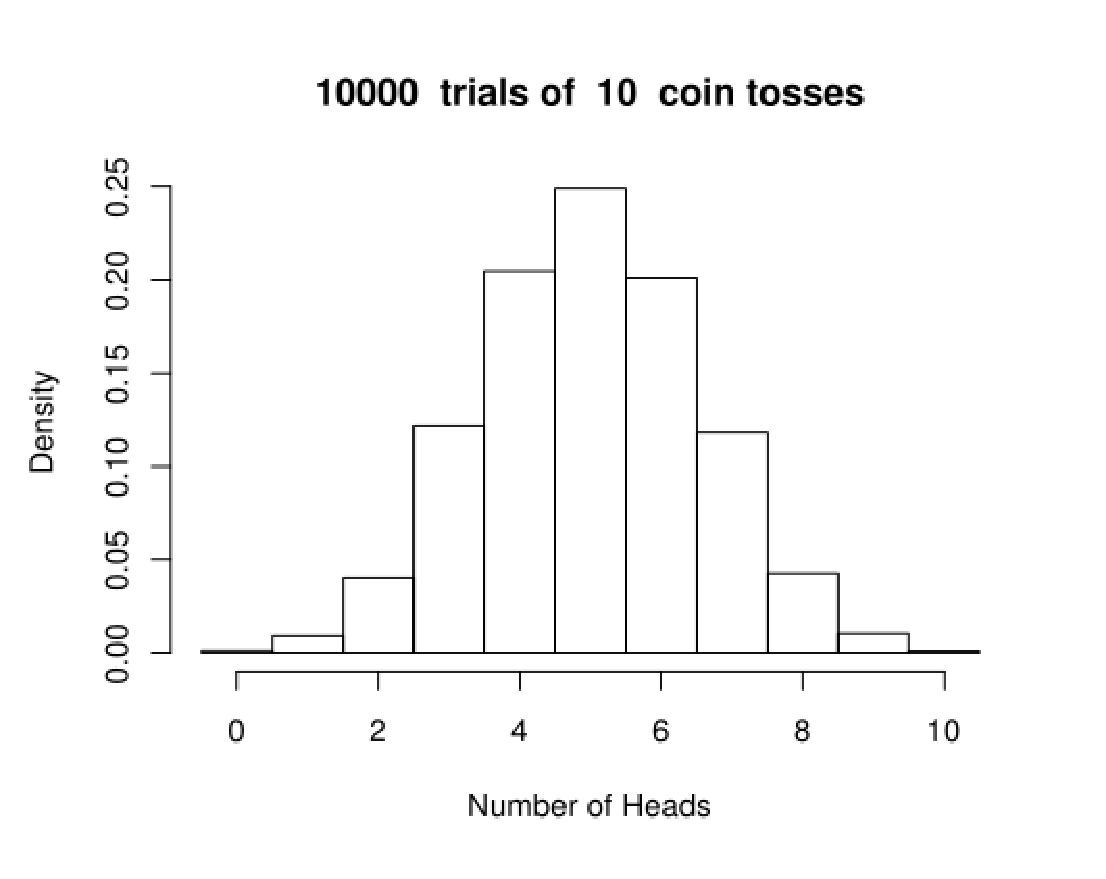
\includegraphics[height=3.7cm]{CoinHistogram.eps}
\end{center}
}
\end{frame}

\subsection{Non-Gaussian Data}
\begin{frame}[t]\frametitle{Non-Gaussian Data}

{\small
\begin{itemize}
\item Not all data follows the normal curve:\\[5pt]
 \texttt{> hist(faithful\$eruptions, breaks=20,}\\
 \texttt{\ \ main="Old Faithful Eruption Durations",}\\
 \texttt{\ \ prob=TRUE, xlab="Duration (min)", ylab="Probability")}\vspace{-10pt}
\end{itemize}
\begin{center}
{\ }\hspace{.1in}
\raisebox{0.4in}{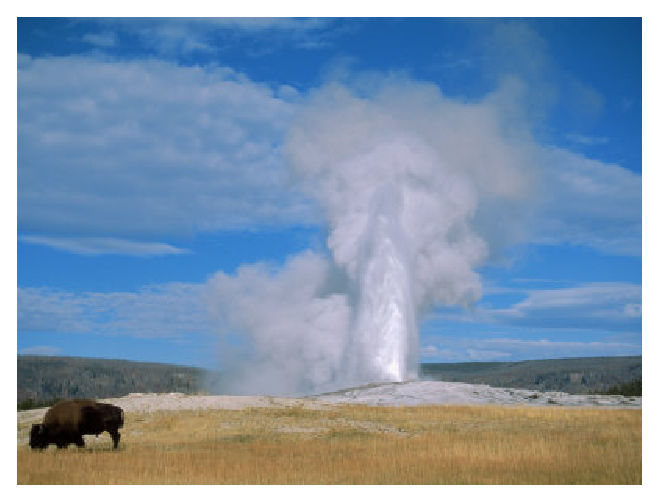
\includegraphics[height=1.2in]{OldFaithful.eps}}\hspace{.2in}
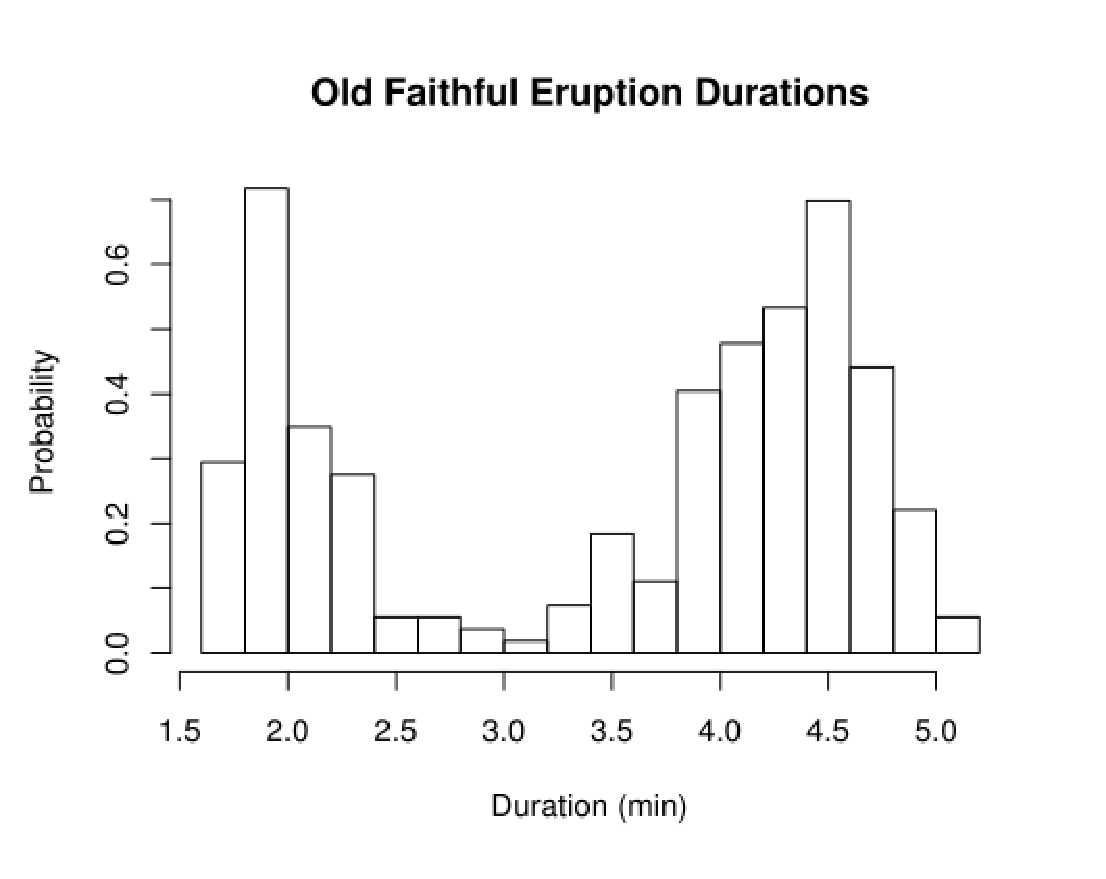
\includegraphics[height=2in]{faithful.eps}
\end{center}
}
\end{frame}


\section{Percentiles}
\subsection{Percentiles}
\begin{frame}[t]\frametitle{Percentiles}
{\small
\begin{itemize}
\item For data that does not follow the normal curve, we use percentiles, quartiles
  and related descriptive statistics to summarize the data.
\item The $25^{th}$ percentile is a number $x$ for which 25\% of the data is 
  less than $x$
\item The $50^{th}$ percentile is a number $x$ for which 50\% of the data is 
  less than $x$ (this is the same as the median)
\item The $75^{th}$ percentile is a number $x$ for which 75\% of the data is 
  less than $x$
\item Use the \texttt{quantile}, \texttt{summary} or \texttt{fivenum} functions in \texttt{R}
  to find quartiles.\\
\texttt{> x <- c(3, 6, 7, 8, 8, 10, 13, 15, 16, 20, 22)}\\
\texttt{> quantile(x)}\\[3pt]
\texttt{{\ }  0\%\ \   25\%\  \ \ 50\%\ \ \   75\%\ \ \   100\%}\\
\texttt{ 3.0\  \  7.5\  \  10.0\ \   15.5\ \  \ 22.0}\\[3pt]
\texttt{> summary(x)}\\
\texttt{{\ } Min\ \ 1st Qu.\ Median\ \ \ Mean\ \ 3rd Qu.\ \ \ Max}\\
\texttt{\ 3.00\ \ \ \ 7.50\ \ \ 10.00\ \  11.64\ \ \ 15.50\ \ 22.00}
\end{itemize}
}

\end{frame}

%
%\section[Normal Percentiles]{Percentiles and the Normal Curve}
%\subsection{Percentiles and the Normal Curve}
%\begin{frame}[t]\frametitle{Percentiles and the Normal Curve}
%{\small
%}
%\end{frame}


\section[Change of Scale]{Change of Scale}
\subsection{Change of Scale}
\begin{frame}[t]\frametitle{Change of Scale}

{\small
\begin{itemize}
\item If you add a number $A$ to each element of a list, then 
   \begin{itemize}
   \item  Mean of new list $=$ $A$ $+$ mean of old list
   \item  sd of new list $=$ sd of old list
   \end{itemize}
\item If you multiply each element of a list by a number $A$, then
   \begin{itemize}
   \item Mean of the new list $=$ $A$ $\times$ mean of old list
   \item sd of new list $=$ $|A|$ $\times$ sd of old list
   \end{itemize}
\item Example:  The mean of the list {\color{blue}$1$, $3$, $4$, $4$, $5$, $7$} is $4$ and the 
          sd is $2$.\\[-10pt]
\hphantom{Example: } The mean of the list {\color{blue}$101$, $103$, $104$, $104$, $105$, $107$} 
  is  $104$ and the sd is $2$.\\[-10pt]
\hphantom{Example: } The mean of the list {\color{blue}$-2$, $-6$, $-8$, $-8$, $-10$, $-14$}
  is $-8$ and the sd is $4$.
\item Example:  For the 100 measurements on Table 1 on p.~99 of our
  text $\mbox{mean}=0.000405$ grams and  $\mbox{sd}=0.000006$ grams.  In ounces,
  the mean is $0.0000142$ and the sd is $2\times 10^{-7}$.
  (1 gm = $0.0352739619$ oz)
\item Example:  The mean of a list of temperature data is $0^{\circ}\mbox{C}$
and the sd is $5^{\circ}\mbox{C}$. This corresponds to a 
  mean of $32^{\circ}\mbox{F}$ and sd of $9^{\circ}\mbox{F}$. 
$\left(\mbox{F}=\frac{9}{5}\,\mbox{C} + 32\right)$
\end{itemize}
}
\label{lastpage}
\end{frame}

\end{document}
